\documentclass[12pt, a4paper]{report}

\usepackage[utf8]{inputenc}
\usepackage[T1]{fontenc}
\usepackage{amsmath}
\usepackage{graphicx}
\usepackage[left=1in, right=1in, top=1in, bottom=1in]{geometry}
\usepackage{array}
\usepackage{booktabs}
\usepackage{caption}
\usepackage{hyperref}
\usepackage{enumitem}
\usepackage{parskip} % For space between paragraphs, no indent
\usepackage{float}   % For [H] option if absolutely needed, otherwise [h!]
\usepackage{setspace} % For line spacing adjustments
\usepackage{titlesec} % For customizing chapter titles
\usepackage{indentfirst}


\titleformat{\chapter}[hang]{\bfseries\Huge}
  {Chapter \thechapter:}{1em}{}

\hypersetup{
    colorlinks=true,        % Bật màu cho liên kết
    linkcolor=blue,         % Màu cho các liên kết nội bộ (nếu có)
    urlcolor=blue,          % Màu cho các liên kết URL
    filecolor=magenta,      % Màu cho liên kết đến file (nếu có)
    pdftitle={My PDF},      % Tiêu đề của PDF (tùy chọn)
    pdfauthor={Author},     % Tác giả của PDF (tùy chọn)
}

% Placeholder for image paths - replace with actual paths if images are available
% \graphicspath{{path/to/your/images/}} % Example

\begin{document}
\setstretch{1.5}  % Giảm khoảng cách giữa các dòng (1.0 là bình thường, giảm xuống < 1.0 sẽ làm chúng gần nhau hơn)

% Trang bìa
\begin{titlepage}
    \begin{center}
       \textbf{\Large POSTS AND TELECOMMUNICATIONS INSTITUTE OF TECHNOLOGY}
    \end{center}
     
    \begin{center}
       \textbf{\Large FACULTY OF INFORMATION TECHNOLOGY I}
    \end{center}
     
    \begin{center}
       \textbf{\Large PYTHON PROGRAMMING COURSE}
    \end{center}
     
    \vspace{1cm}  % Giảm khoảng cách để các phần không quá cách xa nhau
    \begin{center}
       
\includegraphics[width=2in, height=2.5in]{media/logo.png}
    \end{center}
     
    \vspace{1.5cm}  % Điều chỉnh khoảng cách để phần văn bản và bảng cân đối
    \begin{center}
       \textbf{\LARGE ASSIGNMENT REPORT}
    \end{center}
     
    \vspace{1cm}  % Điều chỉnh khoảng cách cho phần bảng
    \begin{center}
       \begin{tabular}{p{4cm} l}
           \textbf{Lecturer}     & : KIM NGOC BACH \\[0.3cm]  % Thêm khoảng cách nhỏ giữa các dòng
           \textbf{Student}      & : DAO VAN KHANG - B23DCVT218\\[0.3cm] 
           \textbf{}             & : VU MINH SANG - B23DCCE082\\[0.3cm] 
           \textbf{Class}        & : D23CQCE04-B \\[0.3cm]
           \textbf{Group}        & : 04 \\[0.3cm]
       \end{tabular}
   \end{center}  
 
    \vfill  % Giữ khoảng cách phía dưới cân đối
    \begin{center}
       \textbf{\large Ha Noi -- 2025}
    \end{center}
 \end{titlepage}

% Tóm tắt
\setlength{\parindent}{2em}  % Bỏ thụt lề
% \setlength{\parskip}{1em}    % Khoảng cách giữa các đoạn

% Chèn phần Summary trước Table of Contents
\cleardoublepage  % Bắt đầu trang mới
\phantomsection  % Đảm bảo tính tương thích với hyperref
\addcontentsline{toc}{chapter}{Summary}  % Thêm phần Summary vào mục lục
\chapter*{Summary}  % Không đánh số cho phần này
This report documents the implementation of Python Programming Assignment 2 for the 2024– 2025 academic year. The objective of the assignment is to perform image classification on the CIFAR-10 dataset by developing, training, and evaluating two distinct neural network architectures using the PyTorch library.

The task is divided into several key stages. The first stage involves model construction: a basic Multi-Layer Perceptron (MLP) neural network with 3 layers will be built, alongside a Convolutional Neural Network (CNN) featuring 3 convolution layers.

The second stage focuses on applying these models to image classification. This includes the complete pipeline of training, validating, and testing both the MLP and CNN on the CIFAR-10 data. As part of the evaluation, learning curves will be plotted to visualize training progress, and confusion matrices will be generated to assess classification performance for each model.

Finally, a comparative analysis will be conducted to discuss and contrast the results obtained from the two neural networks. The project submission will comprise this report in PDF format and the corresponding Python code, delivered via GitHub. 

% Mục lục
\tableofcontents

\setstretch{1.5}  % Giảm khoảng cách giữa các dòng (1.0 là bình thường, giảm xuống < 1.0 sẽ làm chúng gần nhau hơn)

\chapter{Introduction}
Image classification, a fundamental task in computer vision, involves assigning a label or class to an input image from a predefined set of categories. It forms the basis for numerous applications, ranging from autonomous driving and medical image analysis to content-based image retrieval and surveillance systems. The challenge lies in developing algorithms that can effectively learn and generalize visual patterns from raw pixel data to make accurate predictions on unseen images. Over the years, various machine learning approaches have been applied to this problem, with deep learning models, particularly neural networks, demonstrating state-of-the-art performance. 

This project focuses on image classification using the CIFAR-10 dataset.
The CIFAR-10 dataset (Canadian Institute For Advanced Research, 10 classes), accessible at \url{https://www.cs.toronto.edu/~kriz/cifar.html}, is a widely used benchmark collection for computer vision algorithms.
It consists of 60,000 $32 \times 32$ color images in 10 mutually exclusive classes, with 6,000 images per class.
The dataset is pre-divided into 50,000 training images and 10,000 testing images, making it suitable for training and evaluating machine learning models.
The ten classes represent airplanes, automobiles, birds, cats, deer, dogs, frogs, horses, ships, and trucks.

\noindent The primary tasks of this project include:
\begin{itemize}
    \item Building a basic Multi-Layer Perceptron (MLP) neural network with 3 layers.
    \item Building a Convolutional Neural Network (CNN) with 3 convolution layers.
    \item Conducting image classification using both the MLP and CNN, which encompasses training, validation, and testing phases for each model.
    \item Visualizing the training progress and model performance by plotting learning curves and confusion matrices.
    \item Performing a comparative analysis and discussion of the results obtained from the two neural network models.
\end{itemize}

\chapter{Methodology}
This chapter details the procedures and techniques employed for the image classification task on the CIFAR-10 dataset.
It covers dataset preparation, the architectures of the Multi-Layer Perceptron (MLP) and Convolutional Neural Network (CNN) models, the training process, and the metrics used for evaluation.
All implementations were carried out using the PyTorch library.

\section{Dataset Preparation}
\noindent \textbf{Dataset Source and Description :}
\begin{itemize}
    \item The CIFAR-10 dataset was obtained from \url{https://www.cs.toronto.edu/~kriz/cifar-10-python.tar.gz}.
    \item It contains 60,000 $32 \times 32$ color images across 10 classes: \texttt{airplane, automobile, bird, cat, deer, dog, frog, horse, ship, and truck} (6,000 images per class).
    \item The dataset is pre-split into 50,000 training images (in 5 batches) and 10,000 test images (1 batch).
    \item Images are 3-channel (RGB) with $32 \times 32$ pixel dimensions.
\end{itemize}
\textbf{Preprocessing Steps :}
\begin{itemize}
    \item \textbf{Reshaping:} Raw image data was reshaped from flattened arrays (3072 pixels) to a 4D format (Number of images, 3 channels, 32 height, 32 width).
    \item \textbf{Normalization:} Pixel values were normalized using CIFAR-10 specific mean \texttt{(0.4914, 0.4822, 0.4465)} and standard deviation \texttt{(0.2023, 0.1994, 0.2010)}.
    \item \textbf{Data Augmentation (Training Set Only):}
    \begin{itemize}
        \item \texttt{transforms.RandomHorizontalFlip()} : Applied for random horizontal flipping.
        \item \texttt{transforms.RandomCrop(32, padding=4)} : Applied for random cropping after padding.
    \end{itemize}
    \item \textbf{Tensor Conversion:} Images were converted to PyTorch tensors, with pixel values scaled to [0, 1] before normalization.
\end{itemize}
\textbf{Data Splitting :}
\begin{itemize}
    \item The 50,000 training images were split into:
    \begin{itemize}
        \item Training set: 90\% (45,000 images).
        \item Validation set: 10\% (5,000 images).
    \end{itemize}
    \item The 10,000 original test images were used for final model evaluation.
\end{itemize}
$\Rightarrow$ The CIFARDataset was split into:
Training set: 45,000 images (75\%).
Validation set: 5,000 images (8\%).
Test set: 10,000 images (17\%).

\noindent \textbf{Custom Dataset and Data Loaders :}
\begin{itemize}
    \item A \texttt{CIFARDataset} class was implemented for handling images, labels, and transformations.
    \item \texttt{torch.utils.data.DataLoader} was used for batch processing of training, validation, and test datasets.
\end{itemize}

\section{Multi-Layer Perceptron (MLP)}
\noindent    \textbf{Overall Structure :} A 3-layer MLP was built using \texttt{nn.Sequential}.
    Images were first flattened to 3072 features.

\noindent    \textbf{Layer 1 (Hidden) :}
    \begin{itemize}
        \item Linear transformation: \texttt{nn.Linear(3072, 512)}.
        \item Batch normalization: \texttt{nn.BatchNorm1d(512)}.
        \item Activation: \texttt{nn.ReLU()}.
        \item Regularization: \texttt{nn.Dropout(0.3)}.
    \end{itemize}

\noindent    \textbf{Layer 2 (Hidden) :}
    \begin{itemize}
        \item Linear transformation: \texttt{nn.Linear(512, 256)}.
        \item Batch normalization: \texttt{nn.BatchNorm1d(256)}.
        \item Activation: \texttt{nn.ReLU()}.
        \item Regularization: \texttt{nn.Dropout(0.3)}.
    \end{itemize}

\noindent   \textbf{Layer 3 (Output) :}
    \begin{itemize}
        \item Linear transformation: \texttt{nn.Linear(256, 10)} for 10 classes.
    \end{itemize}

\noindent    \textbf{Optimizer and Loss :}
    \begin{itemize}
        \item Optimizer: \texttt{torch.optim.Adam} with a learning rate of \texttt{0.001}.
        \item Loss Function: \texttt{nn.CrossEntropyLoss}.
    \end{itemize}

\section{Convolutional Neural Network (CNN)}
\noindent \textbf{Overall Structure :} A CNN with 3 convolutional layers was built using \texttt{nn.Sequential}.
    
\noindent \textbf{Convolutional Block 1 :}
    \begin{itemize}
        \item Convolution: \texttt{nn.Conv2d(3, 32, kernel\_size=3, padding=1)}.
        \item Activation: \texttt{nn.ReLU()}.
        \item Pooling: \texttt{nn.MaxPool2d(2, 2)} (Output: $32 \times 16 \times 16$).
    \end{itemize}
    
\noindent \textbf{Convolutional Block 2 :}
    \begin{itemize}
        \item Convolution: \texttt{nn.Conv2d(32, 64, kernel\_size=3, stride=1, padding=1)}.
        \item Activation: \texttt{nn.ReLU()}.
        \item Pooling: \texttt{nn.MaxPool2d(2, 2)} (Output: $64 \times 8 \times 8$).
    \end{itemize}
    
\noindent \textbf{Convolutional Block 3 :}
    \begin{itemize}
        \item Convolution: \texttt{nn.Conv2d(64, 128, kernel\_size=3, stride=1, padding=1)}.
        \item Activation: \texttt{nn.ReLU()}.
        \item Pooling: \texttt{nn.MaxPool2d(2, 2)} (Output: $128 \times 4 \times 4$).
    \end{itemize}
    
\noindent \textbf{Fully Connected Layers :}
    \begin{itemize}
        \item Flattening: \texttt{nn.Flatten()} (Input features: 2048).
        \item Dense Layer 1: \texttt{nn.Linear(128*4*4, 1024)} with \texttt{nn.ReLU()} activation.
        \item Dense Layer 2: \texttt{nn.Linear(1024, 512)} with \texttt{nn.ReLU()} activation.
        \item Regularization: \texttt{nn.Dropout(0.3)}.
    \end{itemize}
    
\noindent \textbf{Output Layer :}
    \begin{itemize}
        \item Linear transformation: \texttt{nn.Linear(512, 10)} for 10 classes.
    \end{itemize}
    
\noindent \textbf{Optimizer and Loss :}
    \begin{itemize}
        \item Optimizer: \texttt{torch.optim.Adam} with a learning rate of \texttt{0.001}.
        \item Loss Function: \texttt{nn.CrossEntropyLoss}.
    \end{itemize}

\section{Training Process}
\noindent \textbf{Device :} Training utilized \texttt{cuda} if available, otherwise \texttt{cpu}.
    
\noindent \textbf{Epoch Procedure :} Each epoch consisted of a training loop and a validation loop.
    \begin{itemize}
        \item \textbf{Training Loop:} Model in \texttt{train} mode. Processed batches with forward pass, loss calculation, backpropagation, and optimizer step. Accumulated training loss and accuracy.
        \item \textbf{Validation Loop:} Model in \texttt{eval} mode with \texttt{torch.inference\_mode()}. Processed validation batches for loss and accuracy.
    \end{itemize}
    
    \noindent\textbf{Metrics Recording :} Epoch-wise training/validation accuracy and loss were calculated, stored, and printed.
    
    \noindent \textbf{Hyperparameters :}
    \begin{itemize}
        \item Learning Rate: \texttt{0.001} (Adam optimizer).
        \item Batch Size: \texttt{128} for training, \texttt{256} for validation.
        \item Number of Epochs: \texttt{30} for MLP, \texttt{20} for CNN.
    \end{itemize}

\section{Evaluation Metrics}
\noindent \textbf{During Training/Validation :}
    \begin{itemize}
        \item Loss: \texttt{CrossEntropyLoss}.
        \item Accuracy: Proportion of correctly classified images, calculated as 
        
        \texttt{(preds == y\_batch).sum().item() / y\_batch.size(0)}.
    \end{itemize}
    
    \noindent \textbf{Final Testing (Test Set) :}
    \begin{itemize}
        \item Test Loss: \texttt{CrossEntropyLoss}.
        \item Test Accuracy: Proportion of correctly classified images.
        \item Confusion Matrix: Generated using \texttt{plot\_matrix} from true and predicted labels on the test set to visualize class-wise performance.
    \end{itemize}

\chapter{Results}
This chapter presents the experimental outcomes from training and evaluating the Multi-Layer Perceptron (MLP) and Convolutional Neural Network (CNN) models on the CIFAR-10 dataset.
It includes an analysis of the learning curves, confusion matrices, and a summary of the performance on the test set.

\section{Learning Curves}
Learning curves, which plot the model's performance metrics (loss and accuracy) on the training and validation sets over epochs, are crucial for understanding the learning process and diagnosing potential issues like overfitting or underfitting.

\textbf{MLP Learning Curves :}
\begin{figure}[h!]
    \centering
    % The image source was a base64 string. Using a placeholder.
    % Replace 'mlp_learning_curves.png' with the actual file if available.
    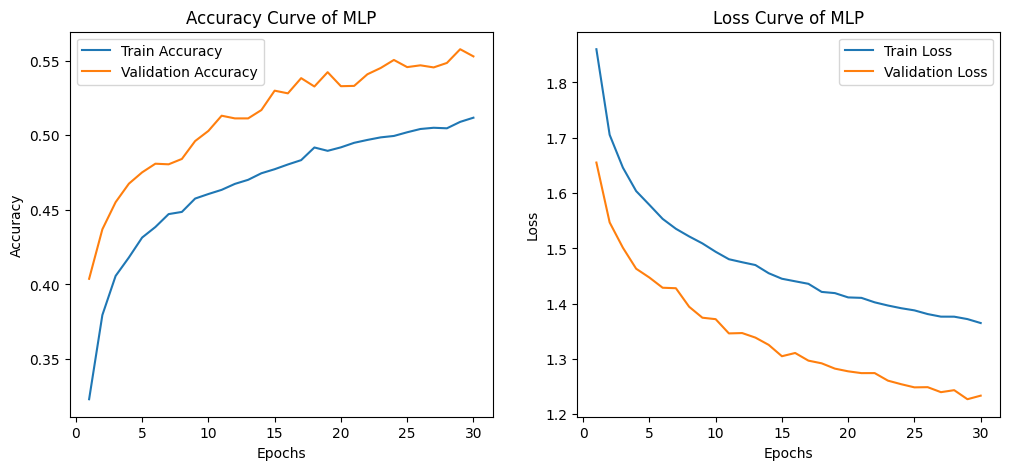
\includegraphics[width=0.9\textwidth]{media/mlp_learning_curves.png} 
    \caption{Accuracy and Loss Curves of MLP.}
    \label{fig:mlp_learning_curves}
\end{figure}

The training curves of the MLP model provide a clear picture of its learning behavior over 30 epochs.
From the accuracy curve, we can see that both the training and validation accuracies increase steadily throughout the training process.
Interestingly, the validation accuracy remains consistently higher than the training accuracy, starting at around 40\% and reaching approximately 56\%, while the training accuracy begins at about 32\% and ends near 51\%.
This trend suggests that the model generalizes well to unseen data and is likely regularized, possibly through techniques such as dropout or weight decay, which help prevent overfitting.

Looking at the loss curves, a similar pattern emerges. Both training and validation losses decrease smoothly over the epochs.
The training loss drops from approximately 1.85 to 1.36, while the validation loss decreases from around 1.65 to 1.22.
The fact that the validation loss remains lower than the training loss throughout is consistent with the accuracy trend and further supports the idea that the model is not overfitting.
In fact, this behavior might indicate slight underfitting or strong regularization, as the model appears to perform better on the validation set than on the training set.

Overall, the MLP model exhibits stable and effective learning, with no signs of overfitting.

\textbf{CNN Learning Curves :}
\begin{figure}[h!]
    \centering
    % The image source was a base64 string. Using a placeholder.
    % Replace 'cnn_learning_curves.png' with the actual file if available.
    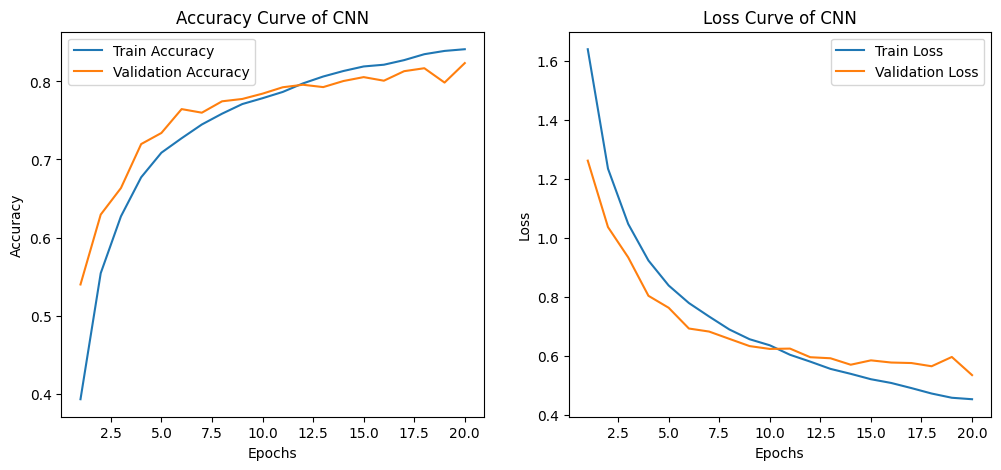
\includegraphics[width=0.9\textwidth]{media/cnn_learning_curves.png}
    \caption{Accuracy and Loss Curves of CNN.}
    \label{fig:cnn_learning_curves}
\end{figure}

The training curves of the CNN model demonstrate strong and consistent learning behavior across 20 epochs.
In the accuracy plot, both the training and validation accuracies show a clear upward trend.
The training accuracy increases from about 40\% to over 85\%, while the validation accuracy starts around 50\% and stabilizes around 83\%.
The close alignment between training and validation accuracy curves indicates that the model is learning effectively without overfitting, and it generalizes well to unseen data.

Similarly, the loss curves further support this observation. The training loss decreases steadily from around 1.6 to approximately 0.42, while the validation loss drops from about 1.35 to 0.5.
Both curves show smooth convergence, and the validation loss remains close to or slightly above the training loss throughout the training process.
This behavior reflects a well-regularized model with no signs of significant overfitting or underfitting.

Overall, the CNN model demonstrates efficient learning with high accuracy and low loss on both training and validation sets.
The stable and closely aligned curves suggest that the model architecture and training strategy are well-tuned.
Further performance gains might be achieved with additional epochs, but the current results already reflect a well-optimized model.

\section{Confusion Matrices}
Confusion matrices provide a detailed breakdown of classification performance for each class, showing the counts of true positive, true negative, false positive, and false negative predictions.

\noindent \textbf{MLP Confusion Matrix :}
\begin{figure}[H]
    \centering
    % The image source was a base64 string. Using a placeholder.
    % Replace 'mlp_confusion_matrix.png' with the actual file if available.
    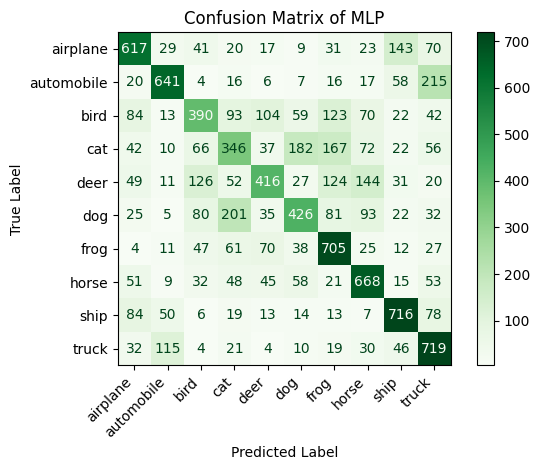
\includegraphics[width=0.6\textwidth]{media/mlp_confusion_matrix.png}
    \caption{Confusion Matrix of MLP.}
    \label{fig:mlp_confusion_matrix}
\end{figure}
  
\begin{table}[H] % Using [H] from float package for "here definitely"
\centering
\caption*{MLP Classification Report} % Unnumbered caption
\begin{tabular}{lrrrr}
\toprule
Class & Precision & Recall & F1-Score & Support \\
\midrule
airplane     & 0.61 & 0.62 & 0.61 & 1000 \\
automobile   & 0.72 & 0.64 & 0.68 & 1000 \\
bird         & 0.49 & 0.39 & 0.43 & 1000 \\
cat          & 0.39 & 0.35 & 0.37 & 1000 \\
deer         & 0.56 & 0.42 & 0.48 & 1000 \\
dog          & 0.51 & 0.43 & 0.47 & 1000 \\
frog         & 0.54 & 0.70 & 0.61 & 1000 \\
horse        & 0.58 & 0.67 & 0.62 & 1000 \\
ship         & 0.66 & 0.72 & 0.69 & 1000 \\
truck        & 0.55 & 0.72 & 0.62 & 1000 \\
\midrule
accuracy     &      &      & 0.56 & 10000 \\
macro avg    & 0.56 & 0.56 & 0.56 & 10000 \\
weighted avg & 0.56 & 0.56 & 0.56 & 10000 \\
\bottomrule
\end{tabular}
\end{table}
\noindent \texttt{MLP Macro Precision: 0.5614} \\
\noindent \texttt{MLP Macro Recall: 0.5644} \\
\noindent \texttt{MLP Macro F1-score: 0.5579}

The Multi-Layer Perceptron (MLP) model achieves an overall \textbf{accuracy of 57\%} on the classification task.
While accuracy provides a general sense of performance, it can mask how well the model performs on individual classes.
To provide a more balanced view, we examine the \textbf{macro-averaged precision (0.5671)}, \textbf{macro-averaged recall (0.5705)}, and \textbf{macro-averaged F1-score (0.5660)}.
These metrics are particularly useful in multi-class settings like this, where each class has equal importance regardless of how frequent it is in the dataset.
\begin{itemize}
    \item \textbf{Macro-averaged precision} is the average of the precision values calculated for each class individually.
It tells us, on average, how many of the predictions for each class were correct.
    \item \textbf{Macro-averaged recall} is the average of the recall scores for all classes, reflecting the model's ability to correctly identify all instances of each class.
    \item \textbf{Macro-averaged F1-score} combines both precision and recall into a single metric per class and then averages them, providing a balanced measure of model quality across all categories.
\end{itemize}

Looking at the individual class performance, the model excels in classes like automobile (F1-score: 0.69) and ship (0.68).
These categories benefit from relatively high recall and precision. For example, "ship" achieves a recall of 0.73, indicating that the model correctly identified 73\% of all ship images, while also maintaining a precision of 0.62, showing that most of the predicted ships were indeed ships.

However, performance drops significantly for visually ambiguous classes. The cat class has an F1-score of just 0.40, with balanced but low precision and recall (both 0.40).
This is consistent with the confusion matrix, where cats are often misclassified as dogs or birds.
Similarly, bird (F1-score: 0.45) and dog (0.46) also exhibit confusion with each other and with related animal categories.
These low scores suggest that the MLP struggles to distinguish subtle features, which is a known limitation of fully connected architectures when applied directly to image data.

Another issue can be seen with the truck and automobile classes, which are often confused with each other.
Despite this, their individual F1-scores (truck: 0.62, automobile: 0.69) remain relatively higher due to decent recall and precision, showing that the model still makes a majority of correct predictions.

In conclusion, while the MLP shows \textbf{reasonable performance on more visually distinct categories}, it struggles with \textbf{fine-grained distinctions among similar classes}, as indicated by both the confusion matrix and the per-class F1-scores.
The macro-averaged metrics help expose these weaknesses by treating each class equally, regardless of how common it is.

\noindent \textbf{CNN Confusion Matrix :}
\begin{figure}[h!]
    \centering
    % The image source was a base64 string. Using a placeholder.
    % Replace 'cnn_confusion_matrix.png' with the actual file if available.
    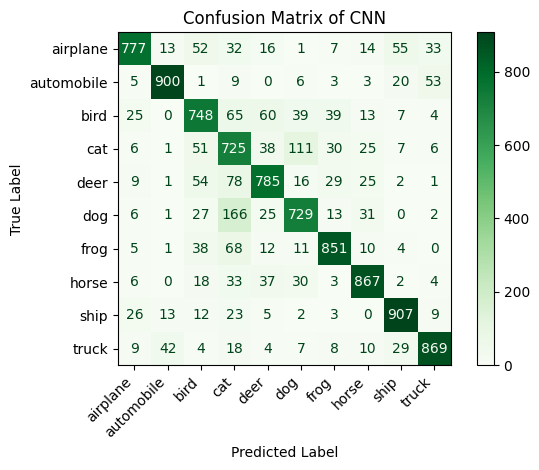
\includegraphics[width=0.7\textwidth]{media/cnn_confusion_matrix.png}
    \caption{Confusion Matrix of CNN.}
    \label{fig:cnn_confusion_matrix}
\end{figure}

\noindent The following table shows the CNN Classification Report:
\begin{table}[H] % Using [H] from float package for "here definitely"
\centering
\caption*{CNN Classification Report} % Unnumbered caption
\begin{tabular}{lrrrr}
\toprule
Class & Precision & Recall & F1-Score & Support \\
\midrule
airplane     & 0.89 & 0.78 & 0.83 & 1000 \\
automobile   & 0.93 & 0.90 & 0.91 & 1000 \\
bird         & 0.74 & 0.75 & 0.75 & 1000 \\
cat          & 0.60 & 0.72 & 0.65 & 1000 \\
deer         & 0.80 & 0.79 & 0.79 & 1000 \\
dog          & 0.77 & 0.73 & 0.75 & 1000 \\
frog         & 0.86 & 0.85 & 0.86 & 1000 \\
horse        & 0.87 & 0.87 & 0.87 & 1000 \\
ship         & 0.88 & 0.91 & 0.89 & 1000 \\
truck        & 0.89 & 0.87 & 0.88 & 1000 \\
\midrule
accuracy     &      &      & 0.82 & 10000 \\
macro avg    & 0.82 & 0.82 & 0.82 & 10000 \\
weighted avg & 0.82 & 0.82 & 0.82 & 10000 \\
\bottomrule
\end{tabular}
\end{table}
\noindent \texttt{CNN Macro Precision: 0.8216}\\
\noindent \texttt{CNN Macro Recall: 0.8158}\\
\noindent \texttt{CNN Macro F1-score: 0.8176}

The CNN model demonstrates commendable overall performance on the CIFAR-10 dataset, achieving an accuracy of \textbf{81\%} and macro average F1-score, precision, and recall all around \textbf{0.81}.
This indicates a strong and relatively balanced ability to classify images across the ten diverse categories.
The model particularly excels with classes that have distinct visual characteristics.
For instance, \textbf{automobile} and \textbf{ship} are identified with exceptional accuracy, boasting \textbf{F1-scores} of \textbf{0.90} and \textbf{0.89} respectively.
The CNN model demonstrates commendable overall performance on the CIFAR-10 dataset, achieving an accuracy of \textbf{81\%} and macro average F1-score, precision, and recall all around \textbf{0.81}.
This indicates a strong and relatively balanced ability to classify images across the ten diverse categories.

Despite these strengths, the CNN model encounters certain challenges, primarily in distinguishing between visually similar classes.
The classic confusion between \textbf{cat} and \textbf{dog} persists as the most notable issue;
the \textbf{cat} class has the lowest precision at \textbf{0.64} and an \textbf{F1-score} of \textbf{0.66}, while the \textbf{dog} class exhibits the lowest recall at \textbf{0.67} with an \textbf{F1-score} of \textbf{0.71}.
The confusion matrix confirms this, revealing that \textbf{101} \textbf{cat} images were misidentified as \textbf{dog}, and a significant \textbf{178} \textbf{dog} images were misclassified as \textbf{cat}.
The \textbf{bird} class also presents some difficulty, with a lower precision of \textbf{0.67}, meaning that while it correctly identifies \textbf{80\%} of true birds recall of 0.80, other animal images are often misclassified as \textbf{bird}.
Furthermore, \textbf{deer} images are sometimes confused with \textbf{bird} and \textbf{horse}, impacting its recall of \textbf{0.72}.
While some confusion also exists between \textbf{automobile} and \textbf{truck}, and \textbf{airplane} and \textbf{ship}, these are considerably less frequent than observed with simpler models.
These detailed metrics, when paired with the visual data from the confusion matrix, provide a clear picture of the CNN's class-specific performance, highlighting its overall effectiveness but also pinpointing specific areas where fine-grained distinctions remain a hurdle.

\section{Performance on Test Set}
The final performance of both models was evaluated on the unseen test set, comprising 10,000 images.
The key metrics are Test Loss, Test Accuracy, and the macro-averaged Precision, Recall, and F1-score.

\begin{table}[H]
\centering
\caption{Summary of Model Performance on the CIFAR-10 Test Set.}
\label{tab:model_performance_summary1}
\begin{tabular}{lrrrrr}
\toprule
Model & Test Loss & Test Accuracy & Precision & Recall & F1-Score \\
\midrule
MLP & 1.2125 & 0.5705 & 0.5671 & 0.5705 & 0.5660 \\
CNN & 0.5723 & 0.8068 & 0.8114 & 0.8068 & 0.8073 \\
\bottomrule
\end{tabular}
\end{table}

As indicated in Table \ref{tab:model_performance_summary1}, the MLP model achieved a test accuracy of 57.05\% with a test loss of 1.2152.
Its macro-averaged precision, recall, and F1-score were approximately 0.5671, 0.5706, and 0.5660, respectively.

The CNN model significantly outperformed the MLP, achieving a test accuracy of 80.68\% with a considerably lower test loss of 0.5723.
The CNN's macro-averaged precision, recall, and F1-score were approximately 0.8114, 0.8068, and 0.8073, respectively.
These higher values across all aggregated metrics underscore the CNN's superior classification capability on this image dataset.

The Precision, Recall, and F1-score (Overall/Macro) metrics provide a more nuanced view of model performance.
These are calculated from the true labels (\texttt{y\_true}) and predicted labels (\texttt{y\_pred}) generated for the test set.
The \texttt{classification\_report} from \texttt{sklearn.metrics} provides these values, and the 'macro avg' figures have been used to populate the table above.

\section{Testing on Non-CIFAR Images from the Internet}
\begin{figure}[h!]
    \centering
    % The image source was a base64 string. Using a placeholder.
    % Replace 'non_cifar_test_images.png' with the actual file if available.
    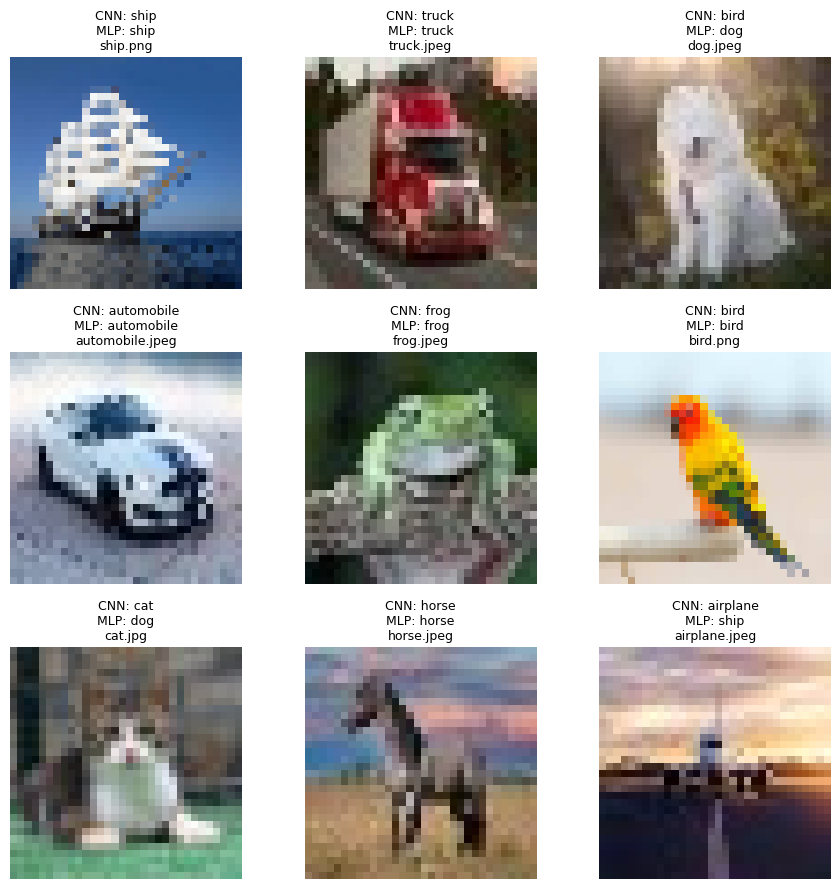
\includegraphics[width=0.8\textwidth]{media/non_cifar_test_images.png}
    \caption{Testing on Non-CIFAR Images from the Internet.}
    \label{fig:non_cifar_images}
\end{figure}

\chapter{Discussion}
This chapter analyzes the performance of the Multi-Layer Perceptron (MLP) and Convolutional Neural Network (CNN) models on the CIFAR-10 dataset, highlighting their comparative strengths, weaknesses, challenges, and areas for potential improvement, based on the provided experimental results.

\section{Comparison of MLP and CNN Results}
\noindent \textbf{Direct Comparison of Performance Metrics}

The final performance of both models on the unseen CIFAR-10 test set is summarized below:

\medskip % Add some vertical space
\noindent\textbf{Table 4.1: Summary of Model Performance on the CIFAR-10 Test Set.}
\begin{center} % Center the table
\begin{tabular}{lrr}
\toprule
Metric & 3-Layer MLP & 3-Convolution-Layer CNN \\
\midrule
Test Accuracy   & 57.05\% & 80.68\% \\
Test Loss       & 1.2125  & 0.5723  \\
Macro Precision & 0.5671  & 0.8114  \\
Macro Recall    & 0.5705  & 0.8068  \\
Macro F1-Score  & 0.5660  & 0.8073  \\
\bottomrule
\end{tabular}
\end{center}
\medskip

The \textbf{Convolutional Neural Network (CNN) significantly outperformed the Multi-Layer Perceptron (MLP)} across all reported metrics.
The CNN achieved a test accuracy of 80.68\% compared to the MLP's 57.05\%, indicating a substantial difference in classification capability.

\noindent The \textbf{learning curves} provide insight into these differing performances:
\begin{itemize}
\item For the \textbf{MLP}, the validation accuracy (peaking around 56\%) consistently remained higher than the training accuracy (ending near 51\%), and validation loss was lower than training loss.
This suggests that the MLP was well-regularized and did not overfit;
however, it might also indicate slight underfitting or that its capacity was insufficient to fully capture the complexity of the image data.
The learning was stable but reached a performance plateau significantly lower than the CNN.

\item The \textbf{CNN's} learning curves showed training and validation accuracies increasing steadily and closely (validation ~83\%, training >85\%).
The loss curves also demonstrated smooth convergence with validation loss remaining close to training loss.
This indicates that the CNN learned effectively from the training data and generalized well to unseen data without significant overfitting, efficiently utilizing its architecture for the task.
\end{itemize}

\noindent The \textbf{confusion matrices} further highlight the CNN's superiority:
\begin{itemize}
\item The \textbf{MLP} confusion matrix revealed widespread confusion between classes, particularly struggling with visually similar categories.
For instance, it achieved low F1-scores for 'cat' (0.40), 'bird' (0.45), and 'dog' (0.46), indicating difficulty in distinguishing subtle features.
While it performed reasonably on more distinct classes like 'automobile' (F1: 0.69) and 'ship' (F1: 0.68), its overall ability to discriminate was limited.

\item The \textbf{CNN} confusion matrix showed a much stronger ability to correctly classify images.
It achieved high F1-scores for distinct classes like 'automobile' (0.90) and 'ship' (0.89).
While it still faced challenges with highly similar classes (e.g., 'cat' F1: 0.66, often confused with 'dog'), its per-class performance was substantially better across the board than the MLP.
\end{itemize}
\textbf{Analysis of Differences in Image Data Processing}

The fundamental reason for the performance disparity lies in how these architectures process image data:
\begin{itemize}
    \item \textbf{MLPs} typically require the input image to be flattened into a one-dimensional vector.
    This process discards the crucial spatial relationships between pixels (e.g., how pixels are arranged to form edges or textures).
    Each pixel is treated as an independent feature, making it very difficult for the MLP to learn local patterns and hierarchical features that are vital for image understanding.
    \item \textbf{CNNs}, by design, preserve and exploit spatial information. Their convolutional layers use filters (kernels) to scan the input image and detect local patterns (like edges, corners, textures) in different parts of the image.
    Subsequent layers can then combine these simpler patterns to learn more complex features and objects.
    Pooling layers help in reducing dimensionality while retaining important information and providing a degree of translation invariance.
    This inherent ability to learn a hierarchy of spatial features makes CNNs exceptionally effective for image-related tasks like classification.
\end{itemize}

\section{Strengths and Weaknesses}
\textbf{MLP}: The 3-layer \textbf{MLP} demonstrated some strengths, such as stable learning and good regularization, as its learning curves indicated stable learning without overfitting, suggesting the regularization techniques (dropout, batch normalization) were effective.
    Additionally, MLPs are generally simpler in concept and implementation compared to CNNs. However, the MLP also exhibited significant weaknesses.
    Its performance was substantially lower in accuracy, precision, recall, and F1-scores compared to the CNN.
    This was largely due to poor feature extraction for images, as the flattening of input images led to a critical loss of spatial information, hindering its ability to learn effective visual representations.
    The learning curves, where validation performance occasionally exceeded training performance, suggest potential underfitting or insufficient model complexity.
    Furthermore, the MLP exhibited significant difficulty in distinguishing visually similar categories, resulting in frequent misclassifications and confusion between classes.

\textbf{Convolution Layer CNN}: The 3 convolution layer CNN exhibited several key strengths, including superior classification performance, achieving a high accuracy of 80.68\% and an F1-score of 0.8073 on the test set.
    It demonstrated effective spatial feature learning by successfully capturing hierarchical spatial features, which led to better discrimination between classes.
    Furthermore, its learning curves indicated good generalization, showing effective learning and robust performance on unseen data.
    The architecture also proved inherently more robust to translations and distortions of features. However, the CNN also had weaknesses.
    It still showed some difficulty with highly similar classes, such as 'cat' versus 'dog', with the 'cat' class having the lowest F1-score (0.66).
    Specific misclassifications were also noted, for instance, classes like 'bird' had lower precision (0.67), and 'deer' images were sometimes confused with other animal classes.
    Finally, CNNs are inherently more complex to design and tune than basic MLPs.

\section{Potential Improvements}
Future work could focus on enhancing model performance through several avenues.
Implementing more advanced CNN architectures like ResNet or VGG, or incorporating attention mechanisms, could yield better results.
Transfer learning from models pre-trained on larger datasets like ImageNet also offers a promising direction.

Further refinements can be achieved by systematic hyperparameter optimization using techniques like grid search, and by exploring different regularization methods beyond dropout and batch normalization, such as L1/L2 weight decay or refined early stopping.
Experimenting with alternative optimizers (e.g., SGD with momentum) and learning rate schedulers could also improve convergence.
Expanding data augmentation with techniques like random rotations, color jittering, Mixup, or Cutout, and specifically addressing class confusions (e.g., between 'cat' and 'dog') through targeted augmentation or specialized loss functions, are also key.

Finally, employing ensemble methods, which combine predictions from multiple models, could boost accuracy and robustness.
A more extensive qualitative analysis, including testing on a broader range of non-CIFAR images and using techniques like Grad-CAM to visualize model attention, would provide deeper insights into the models' decision-making processes and generalization capabilities.

\chapter{Conclusion}
This project focused on developing, training, evaluating, and comparing a 3-layer Multi-Layer Perceptron (MLP) and a 3-convolution-layer Convolutional Neural Network (CNN) for classifying images from the CIFAR-10 dataset using PyTorch.
The key findings confirmed the CNN's superior performance for this task.

The MLP achieved a test accuracy of 57.05\%.
While its training was stable and showed no significant overfitting, its performance indicated potential underfitting or an architectural inability to grasp image complexities, struggling notably with visually similar classes like 'cat' (F1-score: 0.40) and 'bird' (F1-score: 0.45).

In contrast, the CNN demonstrated significantly better results, attaining a test accuracy of 80.68\% with effective learning and good generalization.
Its architecture, adept at preserving and utilizing spatial information through convolutional and pooling layers, allowed for effective hierarchical feature learning and improved class discrimination.
Although it faced minor challenges with highly similar classes (e.g., 'cat' F1-score: 0.66), its overall performance was substantially better than the MLP's across all metrics.

The CIFAR-10 experiment underscores that CNNs are far more suitable for image classification.
Their inherent design for learning spatial feature hierarchies makes them adept at image content analysis, unlike MLPs which lose critical spatial data by flattening images.
This project highlights the necessity of selecting model architectures that align with the data's intrinsic characteristics for optimal results.

\end{document}